\documentclass[11pt,letter,twoside]{mc2011}
%%%%%%%%%%%%%%%%%%%%%%%%%%%%%%%%%%%%%%%%%%%%%%%%%%%%%%%%%%%%%%%%%%%%%%%%%%%%
\usepackage{bm}
\usepackage{amsmath}
\usepackage{amssymb}
\usepackage{microtype}
\usepackage{subfigure}
%\usepackage{booktabs} % \toprule, \midrule, \bottomrule
%%% INCLUDE FILE FOR DEFINITIONS
%%% These may require various packages.

% Shortcuts in regular text
\newcommand{\degs}{\ensuremath{^\circ}}
\newcommand{\EE}[1]{\ensuremath{\times 10^{#1}}}
\newcommand{\ttimes}{\ensuremath{{}\times{}}}
\newcommand{\cclicense}{%
  \smash{\raisebox{-0.45ex}{%
  \setlength{\unitlength}{1em}%
  \begin{picture}(1,1)%
    \put(0.5,0.5){\circle{1}}
    \put(0.5,0.5){\hbox to 0pt{\hss\raisebox{-.45ex}{\tiny\textsf{CC}}\hss}}
  \end{picture}%
  }}%
  \hskip -1em%
  \href{http://creativecommons.org/licenses/by-nc-sa/3.0/}%
  {\ \hskip 1em \textsf{BY-NC-SA}}%
}

%\newcommand{\horizsep}{{\par\noindent\centering\rule[.25ex]{.75\columnwidth}{2pt}\par}}
\newcommand{\horizsep}{\vspace{\baselineskip}\noindent\hspace{\stretch{1}}$
\ast\qquad \ast\qquad \ast\qquad
$ \hspace{\stretch{1}} \vspace{\baselineskip}}
\newcommand{\pytrt}{\textsf{PyTRT}}

% Research
\newcommand{\lop}[1]{\mathcal{L}\!\left[#1\right]}
\newcommand{\lopinv}[2]{\mathcal{I}_{#1}\!\left[#2\right]}
\newcommand{\Dtens}{\mat{D}}
\newcommand{\Etens}{\mat{E}}
\newcommand{\Identitytens}{\mat{I}}
\newcommand{\APone}{AP$_1$}
\newcommand{\Pone}{P$_1$}
\newcommand{\SN}{S$_N$}%{S$_\text{N}$}%{$S_N$}%
\newcommand{\PN}{P$_N$}%{P$_\text{N}$}%{$P_N$}%
\newcommand{\CN}{Crank--Nicolson} %Yes, it's Nic not Nich
\newcommand{\Eddington}{\mathcal{E}} %whatever symbol I decided for Eddington
\newcommand{\RadEn}{E} %whatever symbol I decide for radiation energy
\newcommand{\Sigmatr}{\Sigma_{\mathit{tr}}}

% Program names
\newcommand{\cpp}{\textsf{C\raisebox{0.2ex}{++}}}

% General math shortcuts
\newcommand{\ud}{\mathop{}\!\mathrm{d}}
\newcommand{\pder}[2]{\frac{\partial #1}{\partial #2}}
\newcommand{\oder}[2]{\frac{\mathrm{d} #1}{\mathrm{d} #2}}
\newcommand{\tpder}[2]{{\partial #1}/{\partial #2}} %inlined
\newcommand{\toder}[2]{{\mathrm{d} #1}/{\mathrm{d} #2}} %inlined
\newcommand{\lra}{ \quad \Longrightarrow \quad }
\newcommand{\eexp}{\mathop{}\!\mathrm{e}} % upright ``e'' for exponent
\newcommand{\expp}[1]{\exp\!\left( {#1} \right)} % exp with parentheses
\newcommand{\qeq}{\stackrel{\mathrm{?}}{=}}

% Probability
\newcommand{\expectation}[1]{\mathop{}\!\mathrm{E}\!\left[ #1 \right]}
\DeclareMathOperator{\Var}{Var} % variance

% Asymptotic analysis
\DeclareMathOperator{\Ei}{Ei} % Exponential function
\newcommand{\lapl}[1]{\mathcal{L}[{#1}]} %laplace

%change the Re and Im operators from fancy curly letters
\DeclareMathOperator{\MathOpRe}{Re}
\renewcommand{\Re}{\MathOpRe}
\DeclareMathOperator{\MathOpIm}{Im}
\renewcommand{\Im}{\MathOpIm}

%imaginary ``i'' , upright 'i' or \imath
\newcommand{\iimag}{\mathrm{i}}

% Finite differences
\newcommand{\hot}{\text{h.o.t.}}
\newcommand{\inv}{^{-1}}

% Numerical Linear Algebra
\newcommand{\conj}{^{\ast}} % complex conjugate (transpose)
\newcommand{\norm}[1]{\left\| #1 \right\|} % double pipe
\newcommand{\abs}[1]{\left| #1 \right|} % single pipe
\newcommand{\eps}{\varepsilon}
\DeclareMathOperator{\fl}{fl}

\DeclareMathOperator{\acosh}{arccosh} 

% Define a command to write a nice-looking element, e.g. 4,2 He
\newcommand{\elem}[3]{\ensuremath{{}^{{#1}}_{{#2}}\mathrm{{#3}}}}

% Vector definitions
\newcommand{\mat}[1]{\mathbf{#1}} %matrix is bold upright
\renewcommand{\vec}[1]{\bm{#1}} %vector is bold italic
\newcommand{\op}[1]{\mathsf{#1}} % ``operator'' is sans serif

\newcommand{\vd}{\bm{\cdot}} % slightly bold vector dot
\newcommand{\del}{\vec{\nabla}} % gradient (Del) is bold
\newcommand{\grad}{\vec{\nabla}} % gradient

%\newcommand{\abr}[1]{\langle {#1} \rangle}
\newcommand{\abr}[1]{\left\langle {#1} \right\rangle} % angle brackets for avg.

%% topbox is useful in extended definitions of math terms inside an align
\newcommand{\topbox}[2][0.6]{\parbox[t]{#1\columnwidth}{\raggedright{}#2}}

% commands to make text in math mode appear as zero-width (better-looking
% integrals/sums, e.g.)
% from mathmode.pdf page 74, or Alexander R. Perlis ``A complement to \smash,
% \llap, and \rlap''

\def\mathllap{\mathpalette\mathllapinternal}
	\def\mathllapinternal#1#2{%
	\llap{$\mathsurround=0pt#1{#2}$}%
}
\def\clap#1{\hbox to 0pt{\hss#1\hss}}%
\def\mathclap{\mathpalette\mathclapinternal}%
\def\mathclapinternal#1#2{%
	\clap{$\mathsurround=0pt#1{#2}$}%
}
\def\mathrlap{\mathpalette\mathrlapinternal}%
\def\mathrlapinternal#1#2{%
	\rlap{$\mathsurround=0pt#1{#2}$}%
}

\newcommand{\epsiloncolor}[1]{#1}
\newcommand{\Dtens}{\mat{D}}

\makeatletter
\def\input@path{{/Users/seth/_research/figures/}}
\makeatother
%%%%%%%%%%%%%%%%%%%%%%%%%%%%%%%%%%%%%%%%%%%%%%%%%%%%%%%%%%%%%%%%%%%%%%%%%%%%
\usepackage[numbers,sort&compress]{natbib}

\usepackage{fancyhdr}
\usepackage{lastpage}
\usepackage{graphicx}
\usepackage{color}

\pagestyle{fancy}

\globalmc2011

%%%%%%%%%%%%%%%%%%%%%%%%%%%%%%%%%%%%%%%%%%%%%%%%%%%%%%%%%%%%%%%%%%%%%%%%%%%%
\begin{document}

\title{An Anisotropic Diffusion Approximation to Thermal Radiative
Transfer}

\author{
\textbf{Seth R.~Johnson and Edward W.~Larsen}\\
Department of Nuclear Engineering \& Radiological Sciences\\
University of Michigan \\
2355 Bonisteel Boulevard, Ann Arbor, MI, 48109\\
sethrj@umich.edu; edlarsen@umich.edu
}

\maketitle

\thispagestyle{empty}

\begin{abstract}
This paper describes an anisotropic diffusion (AD) method that uses
transport-calculated AD coefficients to efficiently and accurately solve the
thermal radiative transfer (TRT) equations. By assuming weak gradients and angular moments in the radiation
intensity, we derive an expression for the radiation energy density that
depends on a non-local function of the opacity. This nonlocal function is the
solution of a transport equation that can be solved with a single steady-state
transport sweep once per time step, and the function's second angular moment is
the anisotropic diffusion tensor.
To demonstrate the AD method's efficacy, we model radiation flow down a channel 
in ``flatland'' geometry. 

\keywords{Thermal radiative transfer, Anisotropic diffusion, Flux-limited
diffusion, Hybrid methods, Flatland geometry}

\end{abstract}

\newcommand\authorname{Seth~R.~Johnson and Edward~W.~Larsen}
\newcommand\shorttitlename{Anisotropic diffusion for TRT}

\fancymc2011

%%%%%%%%%%%%%%%%%%%%%%%%%%%%%%%%%%%%%%%%%%%%%%%%%%%%%%%%%%%%%%%%%%%%%%%%%%%%
\section{Introduction}
Thermal radiation is the dominant means of energy transfer in a very hot
material, such as the interior
of a star or the
target of a laser-driven shock experiment. The equations describing thermal
radiative transfer (TRT) are
time-dependent, contain strong nonlinearities, and reside in a large phase
space $(\vec{x}, \vec{\Omega}, h\nu, t)$.
These difficulties make TRT the subject of significant work in methods
development, which typically balances fidelity against computational cost. 
%
%Among high-fidelity methods are Fleck and Cummings' Implicit Monte Carlo
%(IMC) method \cite{Fle1971} and the discrete ordinates (\SN) method
%\cite{Mor1996}. Both of these methods require large amounts of computer time:
%IMC requires large numbers of particles to accurately sample the large phase
%space, and \SN\ has to iteratively ``sweep'' through all spatial cells and all
%angles in the quadrature set. Furthermore, the requirement of storing the full
%time-dependent angular intensity imposes a heavy burden on computer memory: IMC
%must store millions of particles in a ``census'' at the end of the time step,
%and \SN\ must store the calculated intensity in all angles at all spatial
%points. One prevalent low-fidelity method is flux-limited diffusion (FLD)
%\cite{Ols2000}, which uses the diffusion approximation to eliminate the angular
%variable and then applies a correction, the flux limiter, to counteract the
%nonphysical infinite propagation speed of standard time-dependent diffusion.
%Because the assumptions used to derive FLD do not hold in many practical
%situations, and because high-fidelity methods may be unfeasibly expensive,
%there is an impetus for the development of a method that hits a sweet spot
%between accuracy and expense.
%
%One example where true transport methods such as \SN\ can be unfeasible is in
%uncertainty quantification, where large numbers of computer runs produce a
%probability distribution function of some output parameters. The Center for
%RAdiative Shock Hydrodynamics (CRASH) has the goal to assess the predictive
%capability of computer simulations in high energy density systems
%\cite{Crash2010}. A mock-up of this problem serves as the primary test case in
%this work.

Previous work \cite{Lar2009c} formulated a steady-state anisotropic diffusion
(AD) method designed to more accurately model the non-diffusive behavior of
voided channels in the Very High Temperature Reactor.  This paper extends AD
solve the TRT equations for problems containing optically thin channels, as
occur in the simulation of certain radiative shocks \cite{Crash2010}.
By making assumptions about the strength of the gradients and
angular moment of the radiative intensity $I$, we systematically derive an
approximate expression for the scalar intensity $\phi$. The result is an
expression for the radiation flux $\vec{F}$, a function of the local radiation
energy
gradient and a nonlocal anisotropic diffusion tensor. The AD tensor is the
second angular moment of a steady-state, purely absorbing transport problem
with a uniform source.

%%%%%%%%%%%%%%%%%%%%%%%%%%%%%%%%%%%%%%%%%%%%%%%%%%%%%%%%%%%%%%%%%%%%%%%%%%%%
\section{Theory}
We consider the gray TRT equations \cite{Pom1973}, which eliminate the energy
unknown from the
full TRT description by approximating the energy dependence of the opacity
$\sigma$ and integrating over all energies. 
\begin{subequations} \label{eqs:fullGrayTRT}
The radiation field is described by a monoenergetic Boltzmann transport
equation:
\begin{equation} \label{eq:fullGrayTransport2}
  \frac{1}{c} \pder{I}{t}(\vec{x}, \vec{\Omega}, t)
  + \vec{\Omega} \vd \del I(\vec{x}, \vec{\Omega}, t) +
 \sigma(\vec{x}, T) I(\vec{x}, \vec{\Omega}, t)
  = \frac{\sigma(\vec{x}, T) a c [T(\vec{x},t)]^4}{4\pi} 
  + \frac{c Q(\vec{x},t)}{4\pi}
\,,
\end{equation}
and the material energy equation describes the time rate of change in the
material energy:
\begin{equation} \label{eq:fullGrayMaterial}
  \frac{1}{c_v}\pder{T}{t}(\vec{x}, t)
  = \sigma(\vec{x}, T) \int_{4\pi}  I \ud \Omega
    - \sigma(\vec{x}, T) ac [T(\vec{x},t)]^4 
\,.
\end{equation}
\end{subequations}

%The nonlinear Planck function $B$ and the generally nonlinear opacity $\sigma$ 

Integrating Eq.~\eqref{eq:fullGrayTransport2} over all angles gives an
expression for the conservation of energy in the radiation field:
\begin{equation} \label{eq:grayTransportZeroth}
 \frac1c \pder{\phi}{t}(\vec{x}, t)
  + \del \vd \vec{F}(\vec{x}, t) +
 \sigma(\vec{x}, T) \phi(\vec{x}, t)
  = c\sigma(\vec{x}, T) a [T(\vec{x},t)]^4 + cQ(\vec{x},t) \,.
\end{equation}
Here the zeroth angular moment of the radiation intensity is the scalar
intensity,
\begin{equation*}
  \phi(\vec{x}, t) \equiv \int_{4\pi} I(\vec{x}, \vec{\Omega}, t) \ud \Omega\,,
\end{equation*}
which is related to the radiation energy density $E$ by $E = \phi/c$.
The first angular moment of $I$ is the radiation flux,
\begin{equation*}
  \vec{F}(\vec{x}, t) \equiv \int_{4\pi} \vec{\Omega} I(\vec{x}, \vec{\Omega},
  t) \ud \Omega\,.
\end{equation*}

If the right hand side of Eq.~\eqref{eq:fullGrayTransport2} is treated as a known
time-dependent quantity, the integrodifferential Boltzmann equation can be
transformed to an integral transport equation by considering sources and
attenuation along the characteristic ray that passes through the point
$\vec{x}$ along $\vec{\Omega}$ \cite{Pri2010}.
%Neglecting the initial and
%boundary conditions, the integral transport equation is
For simplicity, we consider only the spatiotemporal interior of a problem,
where the contribution of the boundary flux and initial condition are
exponentially small. With the initial and boundary terms neglected, the
integral transport equation is:
\begin{subequations} \label{eqs:integralTrtAngularFlux}
  \begin{equation} \label{eq:integralTrtAngularFluxFull}
    I(\vec{x}, \vec{\Omega}, t)
    =\int_{0}^{\infty}
    \eexp^{ -\tau(\vec{x}, \vec{x} - s \vec{\Omega}, \vec{\Omega}, t)}
    \hat Q(\vec{x} - s \vec{\Omega}, \vec{\Omega}, t-s/c) \ud s\,.
  \end{equation}
  The ``known'' source $\hat Q$ is the right hand side in Eq.~\eqref{eq:fullGrayTransport2},
  \begin{equation} \label{eq:integralTrtSource}
    \hat Q(\vec{x}, \vec{\Omega}, t) =  \frac{\sigma(\vec{x}, T[\vec{x},t]) a c
    [T(\vec{x},t)]^4}{4\pi} + \frac{c Q(\vec{x},t)}{4\pi}\,,
  \end{equation}
  which is evaluated along the characteristic ray at a distance $s$, at the time
  $t-s/c$ at which a particle originating at that point reaches $(\vec{x},t)$.
  The optical thickness of the medium between points $\vec{x}$ and
  $\vec{x}'$ along direction $\vec{\Omega}$ is 
  \begin{equation} \label{eq:integralTrtTauDefinition}
    \tau(\vec{x}, \vec{x}', \vec{\Omega}, t) = \int_{0}^{\norm{\vec{x} -
    \vec{x}'}} \sigma(\vec{x}-s'\vec{\Omega}, t-s'/c) \ud s' \,.
  \end{equation}
\end{subequations}
The opacity $\sigma$ is shown with an implicit dependence on time $t$ because
it is a nonlinear function of the temperature $T(\vec{x},t)$.

Substituting $\hat Q$ into Eq.~\eqref{eq:integralTrtAngularFluxFull} gives
\begin{equation*}
    I(\vec{x}, \vec{\Omega}, t)
    = \frac{1}{4\pi}\int_{0}^{\infty}
    \eexp^{ -\tau(\vec{x}, \vec{x} - s \vec{\Omega}, \vec{\Omega}, t)}
    \left[ \sigma a c T^4 + c Q \right]_{(\vec{x} - s
    \vec{\Omega}, t-s/c)} \ud s\,.
\end{equation*}
The quantity in brackets is just the right-hand side of the conservation
equation~\eqref{eq:grayTransportZeroth}. Replacing it with the left-hand
side, we get
\begin{equation}\label{eq:integralTrtLhs}
    I(\vec{x}, \vec{\Omega}, t)
    = \frac{1}{4\pi}\int_{0}^{\infty}
    \eexp^{ -\tau(\vec{x}, \vec{x} - s \vec{\Omega}, \vec{\Omega}, t)}
    \left[ \sigma \phi + \frac{1}{c} \pder{\phi}{t} +\del \vd \vec{F}
    \right]_{(\vec{x} - s \vec{\Omega}, t-s/c)} \ud s\,.
\end{equation}
We will individually evaluate each constituent term of this integral.

To expand and simplify Eq.~\eqref{eq:integralTrtLhs}, it is necessary to make
an ansatz about
the magnitude of the derivatives and moments of some terms in the transport
equation:
\begin{align*}
  I &= O(\epsiloncolor{1}), &
  \sigma &= O(\epsiloncolor{1}), &
  \del I &= O(\epsiloncolor{\epsilon}), &
  \frac1c\pder{I}{t} &= O(\epsiloncolor{\epsilon}), &
  \frac1c\pder{\sigma}{t} &= O(\epsiloncolor{\epsilon}), &
  \int_{4\pi} \vec{\Omega} I\ud \Omega &= O(\epsiloncolor{\epsilon}).
\end{align*}
These assumptions are different (and admittedly less rigorous) than the set traditionally
used to derive the radiation diffusion equations \cite{Lar1983a}. They will
lead to an approximate expression for the angular intensity that is
\emph{not} linear in angle.

We consider the first term of Eq.~\eqref{eq:integralTrtLhs}: 
\begin{align*}
\lefteqn{\frac{1}{4\pi}\int_{0}^{\infty} \eexp^{ -\int_{0}^{s}
  \sigma(\vec{x}-s'\vec{\Omega}, t-s'/c) \ud s'} \sigma(\vec{x} - s \vec{\Omega}, t-s/c)
\phi(\vec{x} - s \vec{\Omega}, t-s/c) \ud s \,.}\qquad&
\\ 
\intertext{By the fundamental theorem of calculus, this is equal without
approximation to}
&=\frac{1}{4\pi}\int_{0}^{\infty} \left( - \oder{}{s} \eexp^{ -\int_{0}^{s}
  \sigma(\vec{x}-s'\vec{\Omega}, t-s'/c) \ud s'}\right)
\phi(\vec{x} - s \vec{\Omega}, t-s/c) \ud s\,.
\\
\intertext{With integration by parts, assuming that $\phi$ is bounded as
$s\to\infty$, this term is}
    \begin{split}
  &=-\frac{1}{4\pi} \bigg[ 
\eexp^{- \int_{0}^{s} \sigma(\vec{x}-s'\vec{\Omega}, t-s'/c) \ud s'} 
\phi(\vec{x} - s \vec{\Omega}, t-s/c) \bigg|_{0}^{\infty}
\\
&\qquad\qquad- \int_{0}^{\infty} \eexp^{- \int_{0}^{s} \sigma(\vec{x}-s'\vec{\Omega}, t-s'/c) \ud s'}
\oder{}{s} \phi(\vec{x} - s \vec{\Omega}, t-s/c)
\ud s
  \bigg]
    \end{split}
  \\
  &=-\frac{1}{4\pi} \bigg[ 
0 -  
\eexp^0 \phi(\vec{x}, t)
- \int_{0}^{\infty} \eexp^{-\tau(\vec{x}, \vec{x} - s \vec{\Omega}, \vec{\Omega}, t)}
\oder{}{s} \phi(\vec{x} - s \vec{\Omega}, t-s/c)
\ud s
  \bigg]
  \\
 &=\frac{1}{4\pi}\phi(\vec{x}, t)
+ \frac{1}{4\pi}\ \int_{0}^{\infty} \eexp^{-\tau(\vec{x}, \vec{x} - s \vec{\Omega}, \vec{\Omega}, t)}
\oder{}{s} \phi(\vec{x} - s \vec{\Omega}, t-s/c)
\ud s\,,
 \\
 \intertext{or, rewriting the streaming derivative,}
 &=\frac{1}{4\pi}\phi(\vec{x}, t)
+ \frac{1}{4\pi}\ \int_{0}^{\infty} \eexp^{-\tau(\vec{x}, \vec{x} - s
\vec{\Omega}, \vec{\Omega}, t)}
\left[ -\vec{\Omega} \vd \del - \frac1c \pder{}{t} \right] \phi(\vec{x} - s \vec{\Omega}, t-s/c)
\ud s\,.
\end{align*}

So far, no approximations have been made, but the integral involves unknowns at
all spatial points along $s$ at prior points in time. Now, using the
assumptions about the strength of the derivatives, we approximate the
nonlocal unknowns with Taylor series. First, we take a Taylor series in space
and time to find $\phi(\vec{x} - s \vec{\Omega}, t-s/c)$ about $ \phi(\vec{x},
t)$
\begin{align*}
  \phi(\vec{x} - s \vec{\Omega}, t-s/c)
  &\sim
  \phi(\vec{x}, t) - s \vec{\Omega} \vd \del \phi(\vec{x}, t)
  - s\frac{1}{c} \pder{\phi}{t}(\vec{x}, t) + \cdots
  \\
  &= \phi(\vec{x}, t) - s \left[ \vec{\Omega} \vd \del
  + \frac{1}{c} \pder{}{t} \right] \phi(\vec{x}, t) + \cdots
  \\
  &= O(\epsiloncolor{1}) +
  O(\epsiloncolor{\epsilon}) + \cdots\,.
\end{align*}
Second, we take a Taylor series only in time for the opacity $\sigma$ embedded
in the optical thickness $\tau$:
\begin{align*}
  \sigma(\vec{x} - s \vec{\Omega}, t-s/c)
  &\sim
  \sigma(\vec{x} - s \vec{\Omega}, t)
  - s\frac{1}{c} \pder{\sigma}{t}(\vec{x} - s \vec{\Omega}, t) + \cdots
  \\
  &= O(\epsiloncolor{1}) + O(\epsiloncolor{\epsilon}) + \cdots\,.
\end{align*}
The expansion of $\phi$ allows it to be moved outside the integral, and the
expansion of $\sigma$ obviates the storage of all prior $\sigma$:
\begin{multline*}
  \int_{0}^{\infty} \eexp^{- \int_{0}^{s} \sigma(\vec{x}-s'\vec{\Omega}, t-s'/c) \ud s'}
\left[ -\vec{\Omega} \vd \del - \frac1c \pder{}{t} \right] \phi(\vec{x} - s \vec{\Omega}, t-s/c)
\ud s
\\
\sim \int_{0}^{\infty} \eexp^{- \int_{0}^{s} \sigma(\vec{x}-s'\vec{\Omega}, t)
\ud s'} \ud s
\left[ -\vec{\Omega} \vd \del - \frac1c \pder{}{t} \right] \phi(\vec{x}, t)
+ O(\epsilon^2) \,.
\end{multline*}
Therefore, the $\sigma\phi$ component of Eq.~\eqref{eq:integralTrtLhs} is
approximated as
\begin{multline}\label{eq:term1Approx}
  \frac{1}{4\pi}\int_{0}^{\infty} \eexp^{ -\tau(\vec{x}, \vec{x} - s
  \vec{\Omega}, \vec{\Omega}, t)} \sigma(\vec{x} - s \vec{\Omega}, t-s/c)
  \phi(\vec{x} - s \vec{\Omega}, t-s/c) \ud s
  \\
  \sim 
  \frac{1}{4\pi}\underbrace{\phi(\vec{x}, t)}_{O(1)}
  + \frac{1}{4\pi}\int_{0}^{\infty} \eexp^{- \int_{0}^{s} \sigma(\vec{x}-s'\vec{\Omega}, t)
\ud s'} \ud s
\underbrace{\left[ -\vec{\Omega} \vd \del - \frac1c \pder{}{t} \right]}_{O(\epsilon)} \phi(\vec{x}, t)\,.
\end{multline}

The second component of Eq.~\eqref{eq:integralTrtLhs}, the time derivative
term, is treated very much like the first: $\phi$ is expanded about
$(\vec{x},t)$, and $\sigma$ is expanded about $(\vec{x}-s\vec{\Omega},t)$. Thus,
\begin{multline}\label{eq:term2Approx}
  \frac{1}{4\pi}\int_{0}^{\infty} \eexp^{ -\tau(\vec{x}, \vec{x} - s
  \vec{\Omega}, \vec{\Omega}, t)}
  \frac{1}{c} \pder{}{t}\phi(\vec{x} - s \vec{\Omega}, t-s/c) \ud s
 \\
 \sim 
  \frac{1}{4\pi}\int_{0}^{\infty} \eexp^{- \int_{0}^{s} \sigma(\vec{x}-s'\vec{\Omega}, t)
  \ud s'} \ud s
  \underbrace{\frac{1}{c} \pder{}{t}}_{O(\epsilon)}\phi(\vec{x}, t)\,.
\end{multline}
The time derivative in Eq.~\eqref{eq:term2Approx} exactly cancels the time
derivative in Eq.~\eqref{eq:term1Approx} when they are added.

The third $\del \vd \vec{F}$ component of Eq.~\eqref{eq:integralTrtLhs}, which
is the composition of two $O(\epsilon)$ operations, is $O(\epsilon^2)$ and
discarded. Adding the two remaining components together gives the
following approximate
expression for the angular intensity:
\begin{equation} \label{eq:anisotropicIntensity}
  I(\vec{x}, \vec{\Omega}, t) \approx
  \frac{1}{4\pi}\phi(\vec{x}, t) - \left[ \int_{0}^{\infty} \frac{1}{4\pi}
  \eexp^{- \int_{0}^{s} \sigma(\vec{x}-s'\vec{\Omega}, t)
  \ud s'} \ud s\right]
\vec{\Omega} \vd \del \phi(\vec{x}, t) \,.
\end{equation}
Taking the first angular moment of the approximate intensity gives an
approximate expression for the radiation flux $\vec{F}$, which resembles Fick's
law:
\begin{align}\nonumber
  \vec{F}(\vec{x}, t) &= \int_{4\pi} \vec{\Omega} I(\vec{x}, \vec{\Omega}, t) \ud \Omega
  \\\nonumber
  &=
  \frac{1}{4\pi}\phi(\vec{x}, t) \int_{4\pi} \vec{\Omega} \ud \Omega
  \\\nonumber
  &\qquad-  \int_{4\pi} \vec{\Omega} \left[ \int_{0}^{\infty} \frac{1}{4\pi}
  \eexp^{- \int_{0}^{s} \sigma(\vec{x}-s'\vec{\Omega}, t)
  \ud s'} \ud s\right]
\vec{\Omega}  \ud \Omega \vd \del \phi(\vec{x}, t)
\\\nonumber
&\equiv - \left[ \int_{4\pi} (\vec{\Omega} \otimes \vec{\Omega})  f(\vec{x},\vec{\Omega},t)
 \ud \Omega \right] \vd \del \phi(\vec{x}, t)
 \\\label{eq:adFlux}
&\equiv - \Dtens(\vec{x},t) \vd \del \phi(\vec{x}, t)\,,
\end{align}
where $\Dtens$ is the anisotropic diffusion tensor, i.e.,
\begin{equation} \label{eq:dTensorComponents}
  D^{ij}(\vec{x},t) = \int_{4\pi} \Omega_i \Omega_j f(\vec{x}, \vec{\Omega}, t)
  \ud \Omega\,,
\end{equation}
and $f$ satisfies the
``steady-state'' transport equation
\begin{equation} \label{eq:dcoeffTransportEquation}
  \vec{\Omega}\vd \del f(\vec{x},\vec{\Omega},t) + \sigma(\vec{x},t) f(\vec{x},\vec{\Omega},t) =
  \frac{1}{4\pi}\,.
\end{equation}

The anisotropic diffusion tensor $\Dtens(\vec{x},t)$ results from consistent
approximations to the transport equation that do not assume that the intensity
is linear in angle. However, in an infinite homogeneous (or even optically
thick homogeneous) medium, $\Dtens = \mat{I}/3\sigma$, which reduces
Eq.~\eqref{eq:adFlux} to Fick's law. Because the solution $f$ is larger along a
voided channel than orthogonal to it, the primary action of the tensor $\Dtens$
is along an optically thin channel. More importantly, $\Dtens$ remains bounded
in voided regions: it does not ``blow up'' like a standard diffusion
coefficient. Finally, the AD coefficient is spatially continuous, so the
solution $\phi$ will have continuous first derivatives.

The transport problem used to calculate $\Dtens$,
Eq.~\eqref{eq:dcoeffTransportEquation}, describes a purely absorbing medium
with a uniform, isotropic source. It is ``steady-state'' in the sense that $f$
only depends on the current $\sigma$ and not on any prior $f(t)$ or other
function of $t$; there is no time-derivative term in that transport equation.
Additionally, because the problem has no
scattering, and hence no iteratively converging scattering source, \emph{it
takes only one transport sweep to solve}. Furthermore, because only the second
angular moment needs to be calculated, \emph{solving the transport problem
requires no storage of the full angular intensity}: the angular moments can be
accumulated as is done in any steady-state transport code. This feature, which
provides for a minimal computer memory footprint, helps set the AD method apart
from true transport methods such as \SN\ and quasidiffusion.
%If
%$\sigma$ is a constant, then $f=1/4\pi\sigma$ and $\int_{4\pi} \vec{\Omega} f
%\vec{\Omega} \ud \Omega = \mat{I}/3\sigma$, which is the diffusion solution.

%Finally, if we revisit the assumptions used in the derivation of the AD method,
%and compare them to Eqs.~\eqref{eq:anisotropicIntensity}
%and~\eqref{eq:adFlux}, we can see that $I$ is $O(1)$, 

The radiation energy conservation equation~\eqref{eq:grayTransportZeroth}, the
material energy conservation equation~\eqref{eq:fullGrayMaterial}, the
anisotropic diffusion approximation to the radiation flux in
Eq.~\eqref{eq:adFlux}, and the transport
equation~\eqref{eq:dcoeffTransportEquation} describe the continuous AD
equations for TRT. To discretize them in time, we apply the semi-implicit
linear approximation \cite{Lar1988}, which approximates $\sigma(T[t]) \approx
\sigma(T^n)$ for $t^n < t < t^{n+1}$. This approximation means that $\Dtens$ is
treated explicitly using the old $\sigma^n$, and one transport sweep per time
step is needed to calculate the AD tensor.

Cell-centered finite differencing is used to spatially discretize the radiation
equation. Because the off-diagonal terms of $\Dtens$ imply transverse photon
leakage across a cell face, an efficient discretization to account for them is
currently unclear. In the implementation used in the numerical test problem,
the off-diagonal terms are discarded.\footnote{We derived and implemented a
discretization, similar to Gol'din's method \cite{Wie2009}, that stores $\phi$ at both cell centers and
cell edges. The addition of these extra unknowns reduces the computational
efficiency and, from limited testing, appears to change the solution only
slightly.}

To discretize the transport equation~\eqref{eq:dcoeffTransportEquation}, we use
the standard \SN\ formulation with an appropriate quadrature set. Because the
method of characteristics \cite{Ask1982} can exactly calculate the
integral embedded in Eq.~\eqref{eq:adFlux}, it was the obvious (if
computationally arduous) method to use. However, numerical experiments
suggested that the diamond difference method (with flux fix-up using the step
method) yielded $\Dtens$ that were only a few percent different yet saved a
factor of five in computational time. The numerical results presented in this
paper use diamond difference.

%%%%%%%%%%%%%%%%%%%%%%%%%%%%%%%%%%%%%%%%%%%%%%%%%%%%%%%%%%%%%%%%%%%%%%%%%%%%
\section{Numerical Test Problem}

The benchmark solution is Fleck and Cummings' Implicit Monte Carlo
(IMC) method \cite{Fle1971}, implemented
with variance reduction methods and using $10^6$ particles per time step. The
computationally intensive IMC method
correctly prevents photons from exceeding the speed of light, but it is subject
to statistical noise and the semi-implicit linearization error.

Also compared is standard diffusion theory, which uses Fick's law to
approximate the radiation flux by assuming a linear-in-angle intensity:
\begin{equation*}
  \vec{F}_\text{D}^{n+1} = - D^{n} \del \phi^{n+1} 
  = -\frac{1}{3\sigma^{n}} \del \phi^{n+1}\,.
\end{equation*}
The time-dependent diffusion equation incorrectly allows radiation energy to
propagate faster than $c$, as does the anisotropic diffusion equation.

The most important competitor for AD is flux-limited diffusion (FLD)
\cite{Ols2000}, which
reduces the diffusion coefficient where $\del \phi$ is large, preserving the
physical limit of $\norm{\vec{F}} < \phi$.
As implemented, FLD treats the diffusion
coefficient and physics semi-implicitly, and its approximation for the
radiation flux is
\begin{equation*}
  \vec{F}_\text{FLD}^{n+1} = - D^{n} \del \phi^{n+1}  = -\left[ (3\sigma^{n})^2
  + \left( \frac{\norm{\del \phi^{n}}}{\phi^{n}}  \right)^2 \right]^{-1/2}
  \del \phi^{n+1}\,.
\end{equation*}


%%%%%%%%%%%%%%%%%%%%%%%%%%%%%%%%%%%%%%%%%%%%%%%%%%%%%%%%%%%%%%%%%%%%%%%%%%%%
\subsection{Problem description}
One application of the AD method is in the Center for Radiative Shock
Hydrodynamics \cite{Crash2010}, which requires numerous radiation transport simulations
to perform uncertainty quantification. A mock-up of their primary problem
of interest, a radiation shock traveling down a tube filled with xenon, serves
as the primary test case in this work.

The problem models radiation flowing down a pipe in flatland geometry, where
photons are constrained to the plane. (This contrasts 2D geometry, where a gap
extends infinitely into and out of the page.) It uses scaled units with $c=a=1$. Fig.~\ref{fig:crashpipeMaterial}
shows the material layout for the problem.
\begin{figure}[htb]
  \centering
  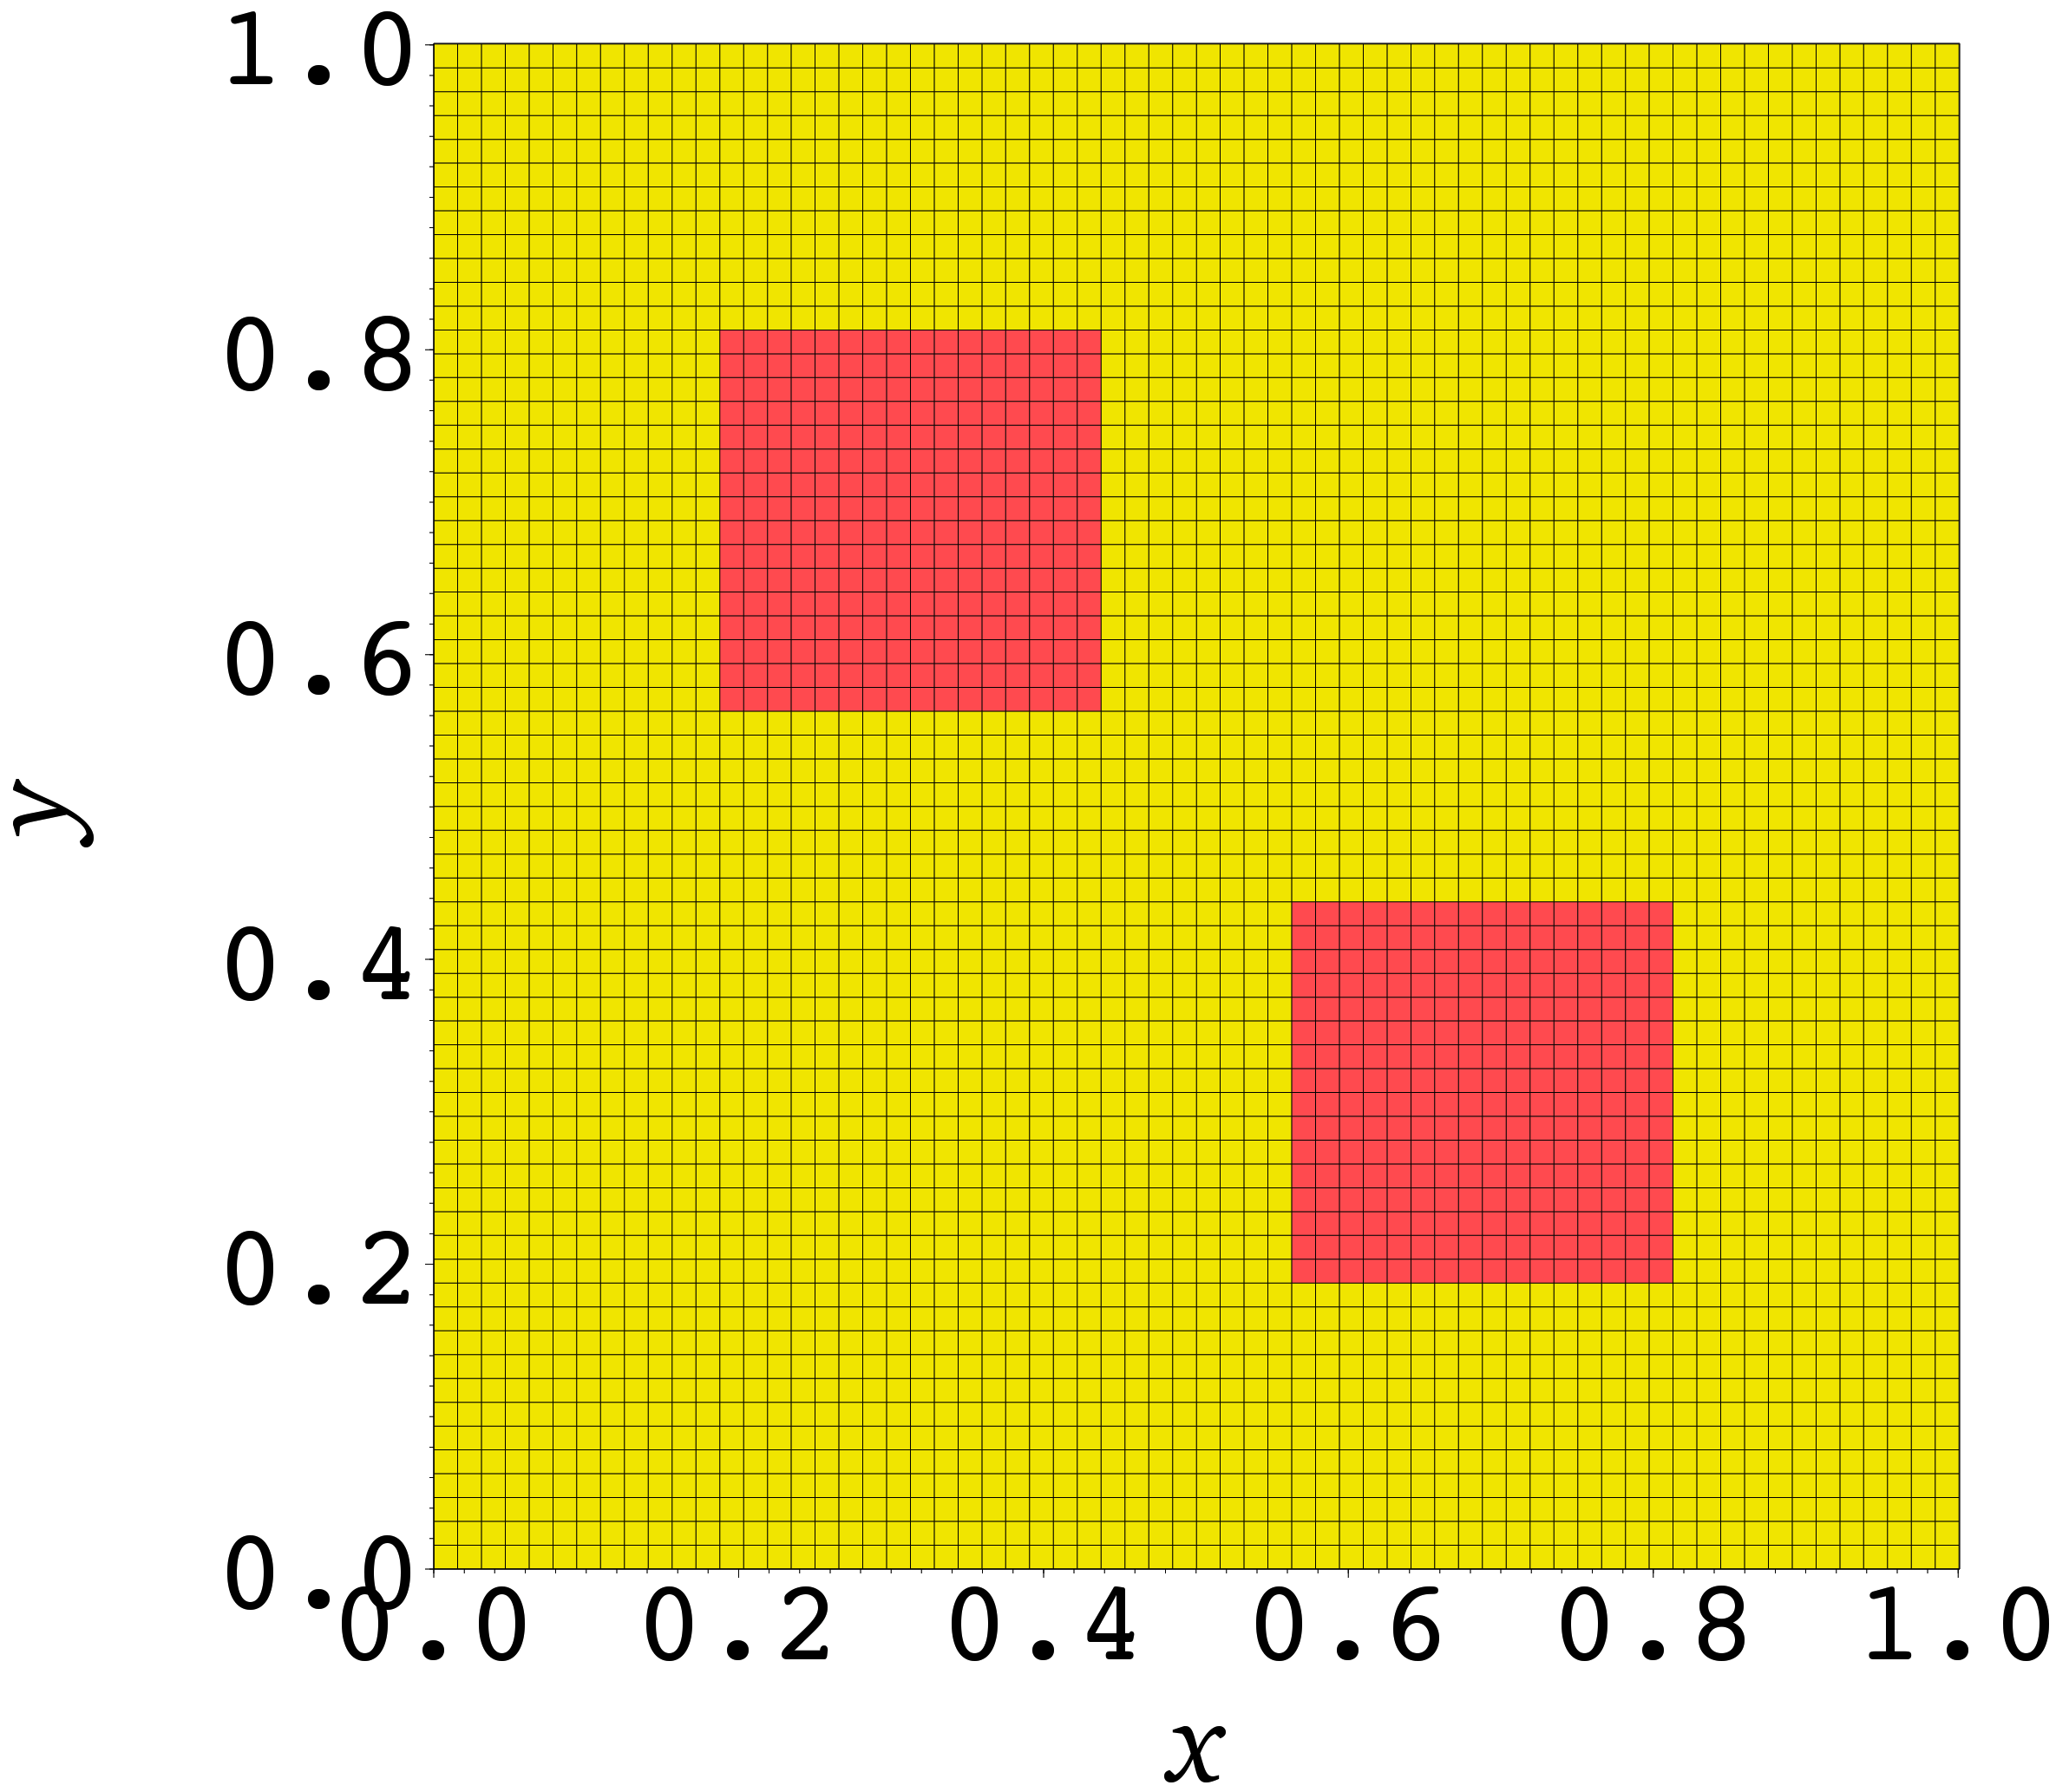
\includegraphics[width=0.75\textwidth]{crashpipe2/materials}
  \caption{Material properties for the pipe problem. The blue square is the
  source, the green channel is a low-opacity region, and the red regions are
  diffusive.}
  \label{fig:crashpipeMaterial}
\end{figure}
The source has a volumetric source
$Q=1$ for $0 \le t \le 1$ and turns off at $t=1$.
That region has $c_v=0.5$ and
$\sigma=0.5$. The diffusive region has a small heat capacity $c_v=0.1$, and an
inverse cubic opacity, $\sigma=T^{-3}$. The streaming channel region has
$c_v=0.1$ and $\sigma=0.01 T^{-3}$. The material temperature and radiation
temperature ($a c T_\text{rad}^4 = \phi$) are $T=T_\text{rad}=0.1$. The left
boundary is reflecting, and the others are vacuum.

The spatial grid is uniform with $\Delta_x=0.1$. The time grid is linearly
increasing and then constant: $\Delta_t(t)\approx 0.1 t + 0.099 (1 - t)$ for $0
\le t < 1$, then $\Delta_t=0.1$ for $1 \le t < 10$. A more resolved time step at
the beginning is a common technique to reduce the effect of the linearization
error (i.e., to prevent a violation of the maximum principle) and to improve
the behavior of the explicitly treated FLD coefficient.

%%%%%%%%%%%%%%%%%%%%%%%%%%%%%%%%%%%%%%%%%%%%%%%%%%%%%%%%%%%%%%%%%%%%%%%%%%%%
\subsection{Results}
Fig.~\ref{fig:mattemp2d} shows the material temperature $T$ at the early time
$t=2$ and the later time $t=10$. The benchmark solution, IMC, correctly
reproduces an important physical features: energy transfer does not exceed the
speed of light, as shown .

\begin{figure}[htb]
  \centering
  \hspace{-1.25in}
  \subfigure[$t=2$]{
  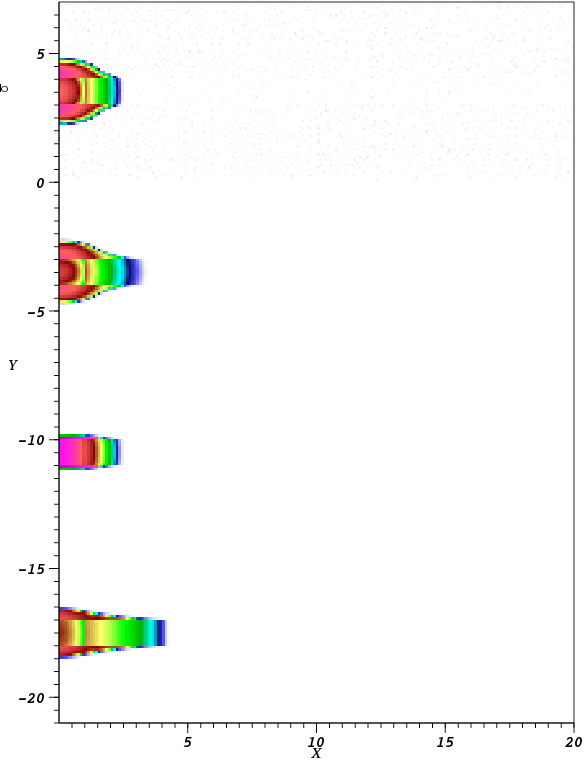
\includegraphics[height=3.5in]{crashpipe2/mattemp2d_t2}}
  \subfigure[$t=10$]{
  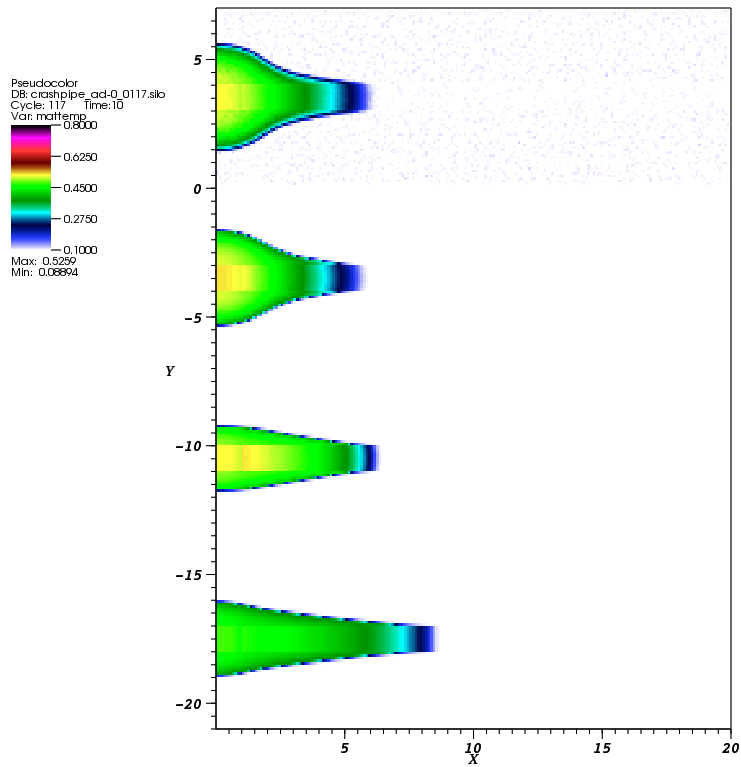
\includegraphics[height=3.5in]{crashpipe2/mattemp_2d0117}}
  \hspace{-1.25in}
  \caption{Pseudocolor plot of material temperature for the four methods (top
  to bottom: IMC, AD, FLD, diffusion).}
  \label{fig:mattemp2d}
\end{figure}

The diffusion coefficient in the heated channel is extremely large and
unphysical, forcing the unphysically rapid transfer of energy throughout the
void. Because the same amount of energy is distributed throughout a larger
region, the overall temperature in the channel is colder, so the penetration
rate into the surrounding diffusive medium is incorrectly small.

Flux-limited diffusion prevents the energy propagation speed from exceeding $c$.
However, it modifies the diffusion coefficients not only in the streaming
region but also in the diffusive region, limiting the spread of radiation into
the walls. As a result, the energy bottles up in the channel.

\begin{figure}[htb]
  \centering
  \hspace{-1.25in}
  \subfigure[$t=1.0$]{
  \small\input{crashpipe2/phi_channel_t1/include.tex}}
  \hspace{-.4in}
  \subfigure[$t=2.0$]{
  \small\input{crashpipe2/phi_channel_t2/include.tex}}
  \hspace{-1.25in}

  \hspace{-1.25in}
  \subfigure[$t=5.0$]{
  \small\input{crashpipe2/phi_channel_t5/include.tex}}
  \hspace{-.4in}
  \subfigure[$t=10.0$]{
  \small\input{crashpipe2/phi_channel_t10/include.tex}}
  \hspace{-1.25in}
  \caption{Scalar intensity along the center of the channel at $t=1,2,5,10$}
  \label{fig:phi}
\end{figure}

\begin{figure}[htb]
  \centering
  \hspace{-1.25in}
  \subfigure[Along the channel centerline]{
  \small\input{crashpipe2/dcoeff_channel_t10/include.tex}}
  \subfigure[Perpendicular to the channel]{
  \hspace{-.4in}
  \small\input{crashpipe2/dcoeff_ortho_t10/include.tex}}
  \hspace{-1.25in}
  \caption{Diffusion coefficients at $t=10$.}
  \label{fig:dcoeffT10}
\end{figure}

%%%%%%%%%%%%%%%%%%%%%%%%%%%%%%%%%%%%%%%%%%%%%%%%%%%%%%%%%%%%%%%%%%%%%%%%%%%%
\clearpage
\section{Conclusions}
The anisotropic diffusion method accounts for some amount of arbitrary
anisotropy in the angular intensity, unlike standard or flux-limited diffusion,
by preserving some transport physics. It works best in problems with weaker
derivatives, as suggested by theory and borne out by numerical experiments.

The currently implemented AD method has several deficiencies whose resolution
could make the method even more accurate. First, we desire to improve the
behavior at the leading edge of the wavefront by limiting the energy
propagation speed to $c$. Additionally, a more careful study of the boundary
and initial conditions should be undertaken. Finally, we should quantify the
penalty of omitting the $D^{xy}$ terms for various problems, or find an
effective discretization scheme that accounts for that transverse leakage.

The AD method could also be made
more computationally efficient by reducing the time spent in transport sweeps,
possibly by
evaluating $\Dtens$ on coarser spatial grid, since it is smooth;
updating $\Dtens$ less frequently than every time step; or
using an advanced quadrature set for \emph{a priori} problem geometries.

Overall, the AD method shows promise for being a computationally efficient
but accurate method for approximately solving the TRT equations.

%%%%%%%%%%%%%%%%%%%%%%%%%%%%%%%%%%%%%%%%%%%%%%%%%%%%%%%%%%%%%%%%%%%%%%%%%%%%
\section*{Acknowledgements}
This material is based upon work supported under a National Science Foundation
Graduate Research Fellowship and a Department of Energy Nuclear
Energy University Programs Graduate Fellowship.

%%%%%%%%%%%%%%%%%%%%%%%%%%%%%%%%%%%%%%%%%%%%%%%%%%%%%%%%%%%%%%%%%%%%%%%%%%%%
%\nocite{Mih1984}
\bibliographystyle{mc}
\bibliography{../SRJall}

%%%%%%%%%%%%%%%%%%%%%%%%%%%%%%%%%%%%%%%%%%%%%%%%%%%%%%%%%%%%%%%%%%%%%%%%%%%%
\end{document}
